
%% Beamer-ported version of mru.tex ==
%% 
%% Original created 05-10-2008; ported to Beamer July 2025
\documentclass{beamer}


\usepackage{xcolor}
\usetheme{Copenhagen}  % Change to Madrid, Copenhagen, etc., for fancier look
% Define custom colors
\definecolor{electricblue}{RGB}{0,191,255} % Electric blue
\definecolor{creamyblue}{RGB}{173,216,230} % Creamy blue
\definecolor{color1574}{rgb}{0.8980392156862745,0.25882352941176473,0.25882352941176473} % Color from PSTricks for tunnel/bus
\newcommand{\red}[1]{\textcolor{red}{#1}}
%\setbeamercolor{structure}{fg=electricblue} % Apply electric blue
\setbeamercolor{structure}{fg=creamyblue} % Apply creamy blue

\usepackage[latin1]{inputenc}
\usepackage{amsmath}
\usepackage{cancel}
\usepackage{tikz}
\usepackage{graphicx}  % For images
\usepackage{lmodern}  % Better font handling to reduce substitution warnings

%%%%%%%%%%%%%%%%%%%%%%%%%%%%%%%%%%%%%
%% Seguridad.. %%%%%%%%%%%%%%%%%%%%%%
\hypersetup{
pdfpagemode={FullScreen},
pdftitle={MRU e41: ver1},
pdfauthor={mmatex.com},
pdfcreator={mmatex.com},
pdfproducer={mmatex.com},
pdfkeywords={Movimiento,Rectilineo,Uniforme}}
%%%%%%%%%%%%%%%%%%%%%%%%%%%%%%%%%%%%%
%%%%%%%%%%%%%%%%%%%%%%%%%%%%%%%%%%%%%

%% You can insert definicions here..

%% DEFINICIONES MIAS..
%\def\psPiFour{12.566371}
%\def\psPiTwo{6.283185}
\def\psPi{3.14159265}
%\def\psPiH{1.570796327}
%\newdimen\pstRadUnit
%\newdimen\pstRadUnitInv
%\pstRadUnit=1.047198cm % this is pi/3
%\pstRadUnitInv=0.95493cm % this is 3/pi

%% Libreria de formulas %%%%%%%%%%%%%%%%%%%%%%%%%%%%%%%%%%%%
\input{lib/FORMULAS}
%% Libreria de Notas    %%%%%%%%%%%%%%%%%%%%%%%%%%%%%%%%%%%%
\input{lib/NOTASUNIDADES}
%%%%%%%%%%%%%%%%%%%%%%%%%%%%%%%%%%%%%%%%%%%%%%%%%%%%%%%%%%%%

%% Titulo y autor .. obligatorio..
\title{MRU e41: ver1}
\subtitle{Otono - 2025}
\author{mmatex.com}

%%%%%%% Para pegar el log.. %%%%%%%%%%%%%%%%%%%%%%%%%%%%%%%
\logo{%
    \begin{tikzpicture}
        \node[opacity=0.2] {
\includegraphics[width=1cm]{images/citlogogrey.eps}}; % Use absolute path if needed: /home/josem/WEB_JJR/libs/figs/citlogogrey.eps
    \end{tikzpicture}
}
%%%%%%%%%%%%%%%%%%%%%%%%%%%%%%%%%%%%%%%%%%%%%%%%%%%%%%%%%%%

%%%%%%%%%%%%%%%%%%%%%%%%%%%%%%%%%%%
%%% Comienzo del documento.. %%%%%%
%%%%%%%%%%%%%%%%%%%%%%%%%%%%%%%%%%%
\begin{document}
\maketitle
%%%%%%%%%%%%%%%%%%%%%%%%%%%%%%%%%%


%________________________________________________________________(ult. col, 65)
% ========================== slide1 ============================= 
\begin{frame}
\frametitle{Movimiento Rectil\'ineo Uniforme}
% 
% -Paragraph1 
%----------------------------------------------------------------
%----------------------------------------------------------------
% -Idea1 
% ============================================================== 
 La f\'ormula principal:

                                                               
% ============================================================== 
% -Idea2 
% ============================================================== 
 
{\huge \vmru}
\vNUa
                                                               
% ============================================================== 
% -Idea3 
% ============================================================== 
                                                               
                                                               
                                                               
% ============================================================== 
%----------------------------------------------------------------
%----------------------------------------------------------------
\end{frame}

%________________________________________________________________(ult. col, 65)
% ========================== slide2 ============================= 
\begin{frame}
\frametitle{MRU}
% 
% -Paragraph1 
%----------------------------------------------------------------
%----------------------------------------------------------------
% -Idea1 
% ============================================================== 

Recu\'erdalo por sus unidades:

% ============================================================== 
% -Idea2 
% ============================================================== 

\begin{equation*}
10\frac{\text{km}}{\text{h}} =
\frac{\text{Se recorren 10 km ({\red distancia})}}
{\text{en 1 hora ({\red tiempo})}}
\end{equation*}
                                                               
% ============================================================== 
% -Idea3 
% ============================================================== 
 
Las otras dos f\'ormulas que se derivan de (\ref{vmru}) son:

{\large \xmru \\ \tmru}
                                                              
% ============================================================== 
%----------------------------------------------------------------
%----------------------------------------------------------------
\end{frame}

%________________________________________________________________(ult. col, 65)
% ========================== slide3 ============================= 
\begin{frame}
\frametitle{MRU}
% 
% -Paragraph1 
%----------------------------------------------------------------
%----------------------------------------------------------------
% -Idea1 
% ============================================================== 
                                                               
Es uniforme porque la velocidad no var\'ia en el tiempo; \\
(v es el mismo en cada unidad de tiempo!)
                                              
% ============================================================== 
% -Idea2 
% ============================================================== 
 
%%%%%%%%%%%%%%%%%%%%%%%%%%%%%
%% Para centrar el grafico %%
\begin{center}
%%%%%%%%%%%%%%%%%%%%%%%%%%%%%
%%%%%%%%%%%%%%%%%%%%%%%%%%%%%

%% Propiedades del grafico.. %%%
%% el eje de X comienza aqui..
\def\iX{0.} %%
\def\iY{0.} %%
%% el eje de y comienza aqui..
\def\jX{8.5} %%
\def\jY{4.5} %%

%%%%%%%%%%%%%%%%%%%%%%%%%%%%%%%%%%%%%%%%%%%%%%%%%%%%%%%%%%%%%%
%% Este es el pspicture enviroment.. el mas sencillo %%%%%%%%%
\begin{tikzpicture}[scale=0.75]
% (x1 , y1  )(x2 , y2)
\draw[->] (0,0) -- (8.5,0) node[below=0.5cm, midway] {t(s)};
\draw[->] (0,0) -- (0,4.5) node[left=0.5cm, midway, rotate=90] {v(cm/s)};

%% Un recta y=ctte .. %%%%%%%
\def\iVctte{2.5}
%% (x1 , y1  )(x2 , y2=y1)
\draw[dashed] (0,\iVctte) -- (8.5,\iVctte);
%%%%%%%%%%%%%%%%%%%%%%%%%%%%%%%%%%%%%%%%%%%%%%%%%%%%%
%%% El do de latex-pstricks!!! %%%%%%%%%%%%%%%%%%%%%%
%%% quiero poner unos punto rojos sobre la recta %%%%
\foreach \iA in {1,2,3,4,5,6,7}{
\fill[red] (\iA,\iVctte) circle (5pt); % Adjusted dotscale to circle radius
}
%\pscircle[fillstyle=solid](\iA,2.5){0.2}}%
%%%%%%%%%%%%%%%%%%%%%%%%%%%%%%%%%%%%%%%%%%%%%%%%%%%%%
%%%%%%%%%%%%%%%%%%%%%%%%%%%%%%%%%%%%%%%%%%%%%%%%%%%%%                                                              
 
%%%%%%%%%%%%%%%%%%%%%%%%%%%%%%%%%%%%%
\end{tikzpicture}
%%%%%%%%%%%%%%%%%%%%%%%%%%%%%%%%%%%%%%%%%%%%%%%%%%%%%%%%%%%%%%
%%%%%%%%%%%%%%%%%%%%%%%%%%%%%%%%%%%%%%%%%%%%%%%%%%%%%%%%%%%%%%

%%%%%%%%%%%%%%%%%%%%%%%%%%%%%%
%% fin centrado del grafico %%
\end{center}
%%%%%%%%%%%%%%%%%%%%%%%%%%%%%%
%%%%%%%%%%%%%%%%%%%%%%%%%%%%%%
                                                              
                                                               
% ============================================================== 
% -Idea3 
% ============================================================== 
                                                               
                                                               
                                                               
% ============================================================== 
%----------------------------------------------------------------
%----------------------------------------------------------------
\end{frame}

%________________________________________________________________(ult. col, 65)
% ========================== slide1 ============================= 
\begin{frame}
\frametitle{MRU}
% 
% -Paragraph1 
%----------------------------------------------------------------
%----------------------------------------------------------------
% -Idea1 
% ============================================================== 
 
Un autob\'us de 75 metros de largo pasa por un t\'unel
de 38 metros de longitud. Si la velocidad del autob\'us
es de 95 km/h, cu\'anto tiempo tarda en salir
completamente del t\'unel?

% ============================================================== 
% -Idea2 
% ============================================================== 
 
\begin{itemize}                                                              

\item El 1er paso en la resoluci\'on de cualquier problema, es la
identificaci\'on de los elementos del problema.            
              
\end{itemize}

% ============================================================== 
%----------------------------------------------------------------
%----------------------------------------------------------------
\end{frame}

%________________________________________________________________(ult. col, 65)
% ========================== slide1 ============================= 
\begin{frame}
\frametitle{MRU}
% 
% -Paragraph1 
%----------------------------------------------------------------
% ============================================================== 
% -Idea1 
% ============================================================== 
 
%% Dibuja una cajita!! %%%%%%%%%%%%%%%%%%%
%% el background de gris..
\fcolorbox{black}{lightgray}{
\begin{tabular}{c}
%%%%%%%%%%%%%%%%%%%%%%%%%%%%%%%%%%%%%%%%%%

{\bf Elementos del Problema}\\

$t=?$	\\

$v=95~\text{km/h}$ \\

$x=$.. Este problema tiene un {\it truquito}! \\
    La distancia que se debe recorrer \\
    para que el autob\'us se considere \\
    completamente fuera \\
    del t\'unel es: 113 metros\\
    Ve la figura que sigue :) 

%%%%%%%%%%%%%%%%%%%%%%%%%%%%%%%%%%%%%%%%%%
\end{tabular}
}
%%%%%%%%%%%%%%%%%%%%%%%%%%%%%%%%%%%%%%%%%%

% Generated with LaTeXDraw 2.0.0
% Fri Aug 01 20:56:48 CEST 2008
% \usepackage[usenames,dvipsnames]{pstricks}
% \usepackage{epsfig}
% \usepackage{pst-grad} % For gradients
% \usepackage{pst-plot} % For axes
\scalebox{1} % Change this value to rescale the drawing.
{
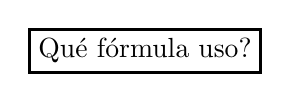
\begin{tikzpicture}
\node[draw, line width=0.04cm] at (10.2,4) {Qu\'e f\'ormula uso?};
\end{tikzpicture}
}

% ============================================================== 
%----------------------------------------------------------------
%----------------------------------------------------------------
\end{frame}

%________________________________________________________________(ult. col, 65)
% ========================== slide2 ============================= 
\begin{frame}
\frametitle{MRU}
% 
% -Paragraph1 
%----------------------------------------------------------------
%----------------------------------------------------------------
% -Idea1 
% ==============================================================

% Generated with LaTeXDraw 2.0.0
% Fri Aug 08 17:58:11 CEST 2008
% Converted from PSTricks to TikZ
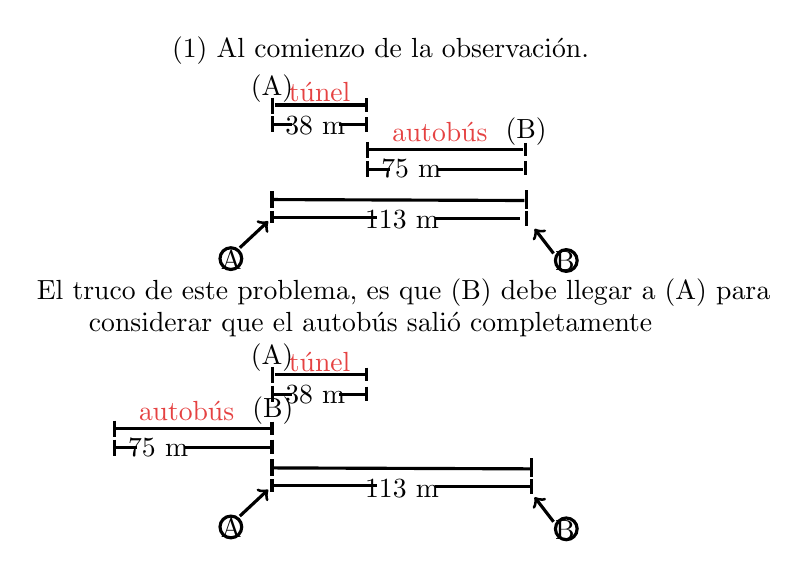
\begin{tikzpicture}[scale=0.6]
% Define color from PSTricks
\definecolor{color1574}{rgb}{0.8980392156862745,0.25882352941176473,0.25882352941176473}

% Tunnel at initial position (top)
\draw[line width=0.04cm] (5.4953127,3.68625) -- (7.3953123,3.68625);
\draw[line width=0.04cm] (5.4553127,3.84625) -- (5.4553127,3.50625);
\draw[line width=0.04cm] (7.4353123,3.82625) -- (7.4353123,3.54625);
\draw[line width=0.04cm] (5.4553127,3.44625) -- (5.4553127,3.10625);
\draw[line width=0.04cm] (5.4553127,3.26625) -- (5.8553123,3.26625);
\draw[line width=0.04cm] (6.8553123,3.26625) -- (7.4153123,3.26625);
\draw[line width=0.04cm] (7.4353123,3.42625) -- (7.4353123,3.12625);
\node[color=color1574] at (6.4439063,3.95625) {t\'unel};
\node at (6.352031,3.25625) {38 m};
\node at (5.43375,4.03625) {(A)};
\node at (7.73375,4.83625) {(1) Al comienzo de la observaci\'on.};

% Bus at initial position (below tunnel)
\draw[line width=0.04cm] (7.4953127,2.74625) -- (10.755313,2.74625);
\draw[line width=0.04cm] (7.4553127,2.90625) -- (7.4553127,2.56625);
\draw[line width=0.04cm] (10.795313,2.88625) -- (10.795313,2.60625);
\draw[line width=0.04cm] (7.4553127,2.50625) -- (7.4553127,2.16625);
\draw[line width=0.04cm] (7.4553127,2.33125) -- (7.9353123,2.33125);
\draw[line width=0.04cm] (8.935312,2.33125) -- (10.755313,2.33125);
\draw[line width=0.04cm] (10.795313,2.50625) -- (10.795313,2.20625);
\node[color=color1574] at (8.987187,3.11625) {autob\'us};
\node at (8.385157,2.33625) {75 m};
\node at (10.81375,3.11625) {(B)};

% Tunnel at final position (middle)
\draw[line width=0.04cm] (5.4953127,-2.01375) -- (7.3953123,-2.01375);
\draw[line width=0.04cm] (5.4553127,-1.85375) -- (5.4553127,-2.19375);
\draw[line width=0.04cm] (7.4353123,-1.87375) -- (7.4353123,-2.15375);
\draw[line width=0.04cm] (5.4553127,-2.25375) -- (5.4553127,-2.59375);
\draw[line width=0.04cm] (5.4553127,-2.43375) -- (5.8553123,-2.43375);
\draw[line width=0.04cm] (6.8553123,-2.43375) -- (7.4153123,-2.43375);
\draw[line width=0.04cm] (7.4353123,-2.27375) -- (7.4353123,-2.57375);
\node[color=color1574] at (6.4439063,-1.74375) {t\'unel};
\node at (6.352031,-2.44375) {38 m};
\node at (5.43375,-1.66375) {(A)};

% Bus at final position (left of tunnel)
\draw[line width=0.04cm] (2.1353126,-3.15375) -- (5.3953123,-3.15375);
\draw[line width=0.04cm] (2.0953126,-2.99375) -- (2.0953126,-3.33375);
\draw[line width=0.04cm] (5.4353123,-3.01375) -- (5.4353123,-3.29375);
\draw[line width=0.04cm] (2.0953126,-3.39375) -- (2.0953126,-3.73375);
\draw[line width=0.04cm] (2.0953126,-3.56875) -- (2.5753126,-3.56875);
\draw[line width=0.04cm] (3.5753126,-3.56875) -- (5.3953123,-3.56875);
\draw[line width=0.04cm] (5.4353123,-3.39375) -- (5.4353123,-3.69375);
\node[color=color1574] at (3.6271875,-2.78375) {autob\'us};
\node at (3.0251563,-3.56375) {75 m};
\node at (5.45375,-2.78375) {(B)};

% Total distance (113 m) at final position
\draw[line width=0.04cm] (5.4353123,-3.99375) -- (10.895312,-4.01375);
\draw[line width=0.04cm] (10.935312,-3.79375) -- (10.935312,-4.19375);
\draw[line width=0.04cm] (5.4353123,-3.81375) -- (5.4353123,-4.17375);
\draw[line width=0.04cm] (5.4353123,-4.23375) -- (5.4353123,-4.49375);
\draw[line width=0.04cm] (5.4753127,-4.37375) -- (7.6553125,-4.37375);
\draw[line width=0.04cm] (8.895312,-4.39375) -- (10.895312,-4.39375);
\draw[line width=0.04cm] (10.935312,-4.23375) -- (10.935312,-4.55375);
\node at (8.1875,-4.42375) {113 m};

% Points A and B at final position (bottom)
\draw[line width=0.04cm] (4.5653124,-5.24375) circle (0.23);
\node at (4.5759373,-5.26375) {A};
\draw[line width=0.04cm,->] (4.7553124,-5.01375) -- (5.3553123,-4.45375);
\draw[line width=0.04cm] (11.665313,-5.28375) circle (0.23);
\node at (11.634687,-5.30375) {B};
\draw[line width=0.04cm,->] (11.395312,-5.13375) -- (10.995313,-4.61375);

% Total distance (113 m) at initial position (top)
\draw[line width=0.04cm] (5.4353123,1.68625) -- (10.775312,1.66625);
\draw[line width=0.04cm] (10.815312,1.88625) -- (10.815312,1.48625);
\draw[line width=0.04cm] (5.4353123,1.86625) -- (5.4353123,1.50625);
\draw[line width=0.04cm] (5.4353123,1.44625) -- (5.4353123,1.18625);
\draw[line width=0.04cm] (5.4753127,1.30625) -- (7.6553125,1.30625);
\draw[line width=0.04cm] (8.895312,1.28625) -- (10.6953125,1.28625);
\draw[line width=0.04cm] (10.815312,1.44625) -- (10.815312,1.12625);
\node at (8.1875,1.25625) {113 m};

% Points A and B at initial position (top)
\draw[line width=0.04cm] (4.5653124,0.43625) circle (0.23);
\node at (4.5759373,0.41625) {A};
\draw[line width=0.04cm,->] (4.7553124,0.66625) -- (5.3553123,1.22625);
\draw[line width=0.04cm] (11.665313,0.39625) circle (0.23);
\node at (11.634687,0.37625) {B};
\draw[line width=0.04cm,->] (11.395312,0.54625) -- (10.995313,1.06625);

% Explanatory text
\node at (8.219531,-0.28375) {El truco de este problema, es que (B) debe llegar a (A) para};
\node at (7.523281,-0.96375) {considerar que el autob\'us sali\'o completamente};
\end{tikzpicture}

% ============================================================== 
%----------------------------------------------------------------
%----------------------------------------------------------------
\end{frame}

%________________________________________________________________(ult. col, 65)
% ========================== slide2 ============================= 
\begin{frame}
\frametitle{MRU}
% 
% -Paragraph1 
%----------------------------------------------------------------
%----------------------------------------------------------------
% -Idea1 
% ============================================================== 
 
{\huge                
\tmru
}                                             
 
% ============================================================== 
% -Idea2 
% ============================================================== 

Pero.. siempre debemos trabajar en el mismo sistema de unidades.
Es decir, si hay un km/h,
debemos transformar los km a m, as\'i como las horas
a segundos :) \\ 

%%%%%%%%%%%%%%%%%%%%%%%%%%%%%%%%%%%%%%%%%%%%%%%%%%%%%%%%%%%%%%%%
%%%%%%%%%%%%%%%%% Cajita de Texto sencilla %%%%%%%%%%%%%%%%%%%%%
\begin{center}
\fcolorbox{red}{white}{
\parbox[c]{5cm}{
1 km = 1000 metros \\
y \\
1 hora = 3600 segundos \\
}}
\end{center}
%%%%%%%%%%%%%%%%%%%%%%%%%%%%%%%%%%%%%%%%%%%%%%%%%%%%%%%%%%%%%%%%
%%%%%%%%%%%%%%%%%%%%%%%%%%%%%%%%%%%%%%%%%%%%%%%%%%%%%%%%%%%%%%%%
                           
% ============================================================== 
% -Idea3 
% ============================================================== 
 
Finalmente..                                                              
                                                               
                                                               
% ============================================================== 
%----------------------------------------------------------------
%----------------------------------------------------------------
\end{frame}

%________________________________________________________________(ult. col, 65)
% ========================== slide3 ============================= 
\begin{frame}
\frametitle{MRU}
% 
% -Paragraph1 
%----------------------------------------------------------------
% ============================================================== 
% -Idea1
% ==============================================================
{\large
\begin{equation} 
t=
\frac{113~\cancel{\text{m}}}{95 \left(\frac{1000}{3600}\right)~\cancel{\text{m}}/\text{s}}=
4.28~\text{s}
\end{equation}
}

                               
% ============================================================== 
% -Idea2 
% ============================================================== 
 
{\large
El tiempo que se demora el punto (B) en llegar a (A) 
es: \fbox{4.28 s}

ps: recuerda; la distancia entre (A) y (B) 
es 113 metros
}

% ============================================================== 
%----------------------------------------------------------------
%----------------------------------------------------------------
\end{frame}

%%%%%%%%%%%%%%%%%%%%%%%%%%%%%%%%%%%%%%%%%%%%%%%%%%%%%%
%%%%%%%%%%%%%%%  Tail %%%%%%%%%%%%%%%%%%%%%%%%%%%%%%%
%%%%%%%%%%%%%%%%%%%%%%%%%%%%%%%%%%%%%%%%%%%%%%%%%%%%%%

\end{document}
%%
%% End of Beamer-ported file ==
%%
%% Modified 05-10-2008
